

\begin{figure*}[!t]
\small
  \centering
  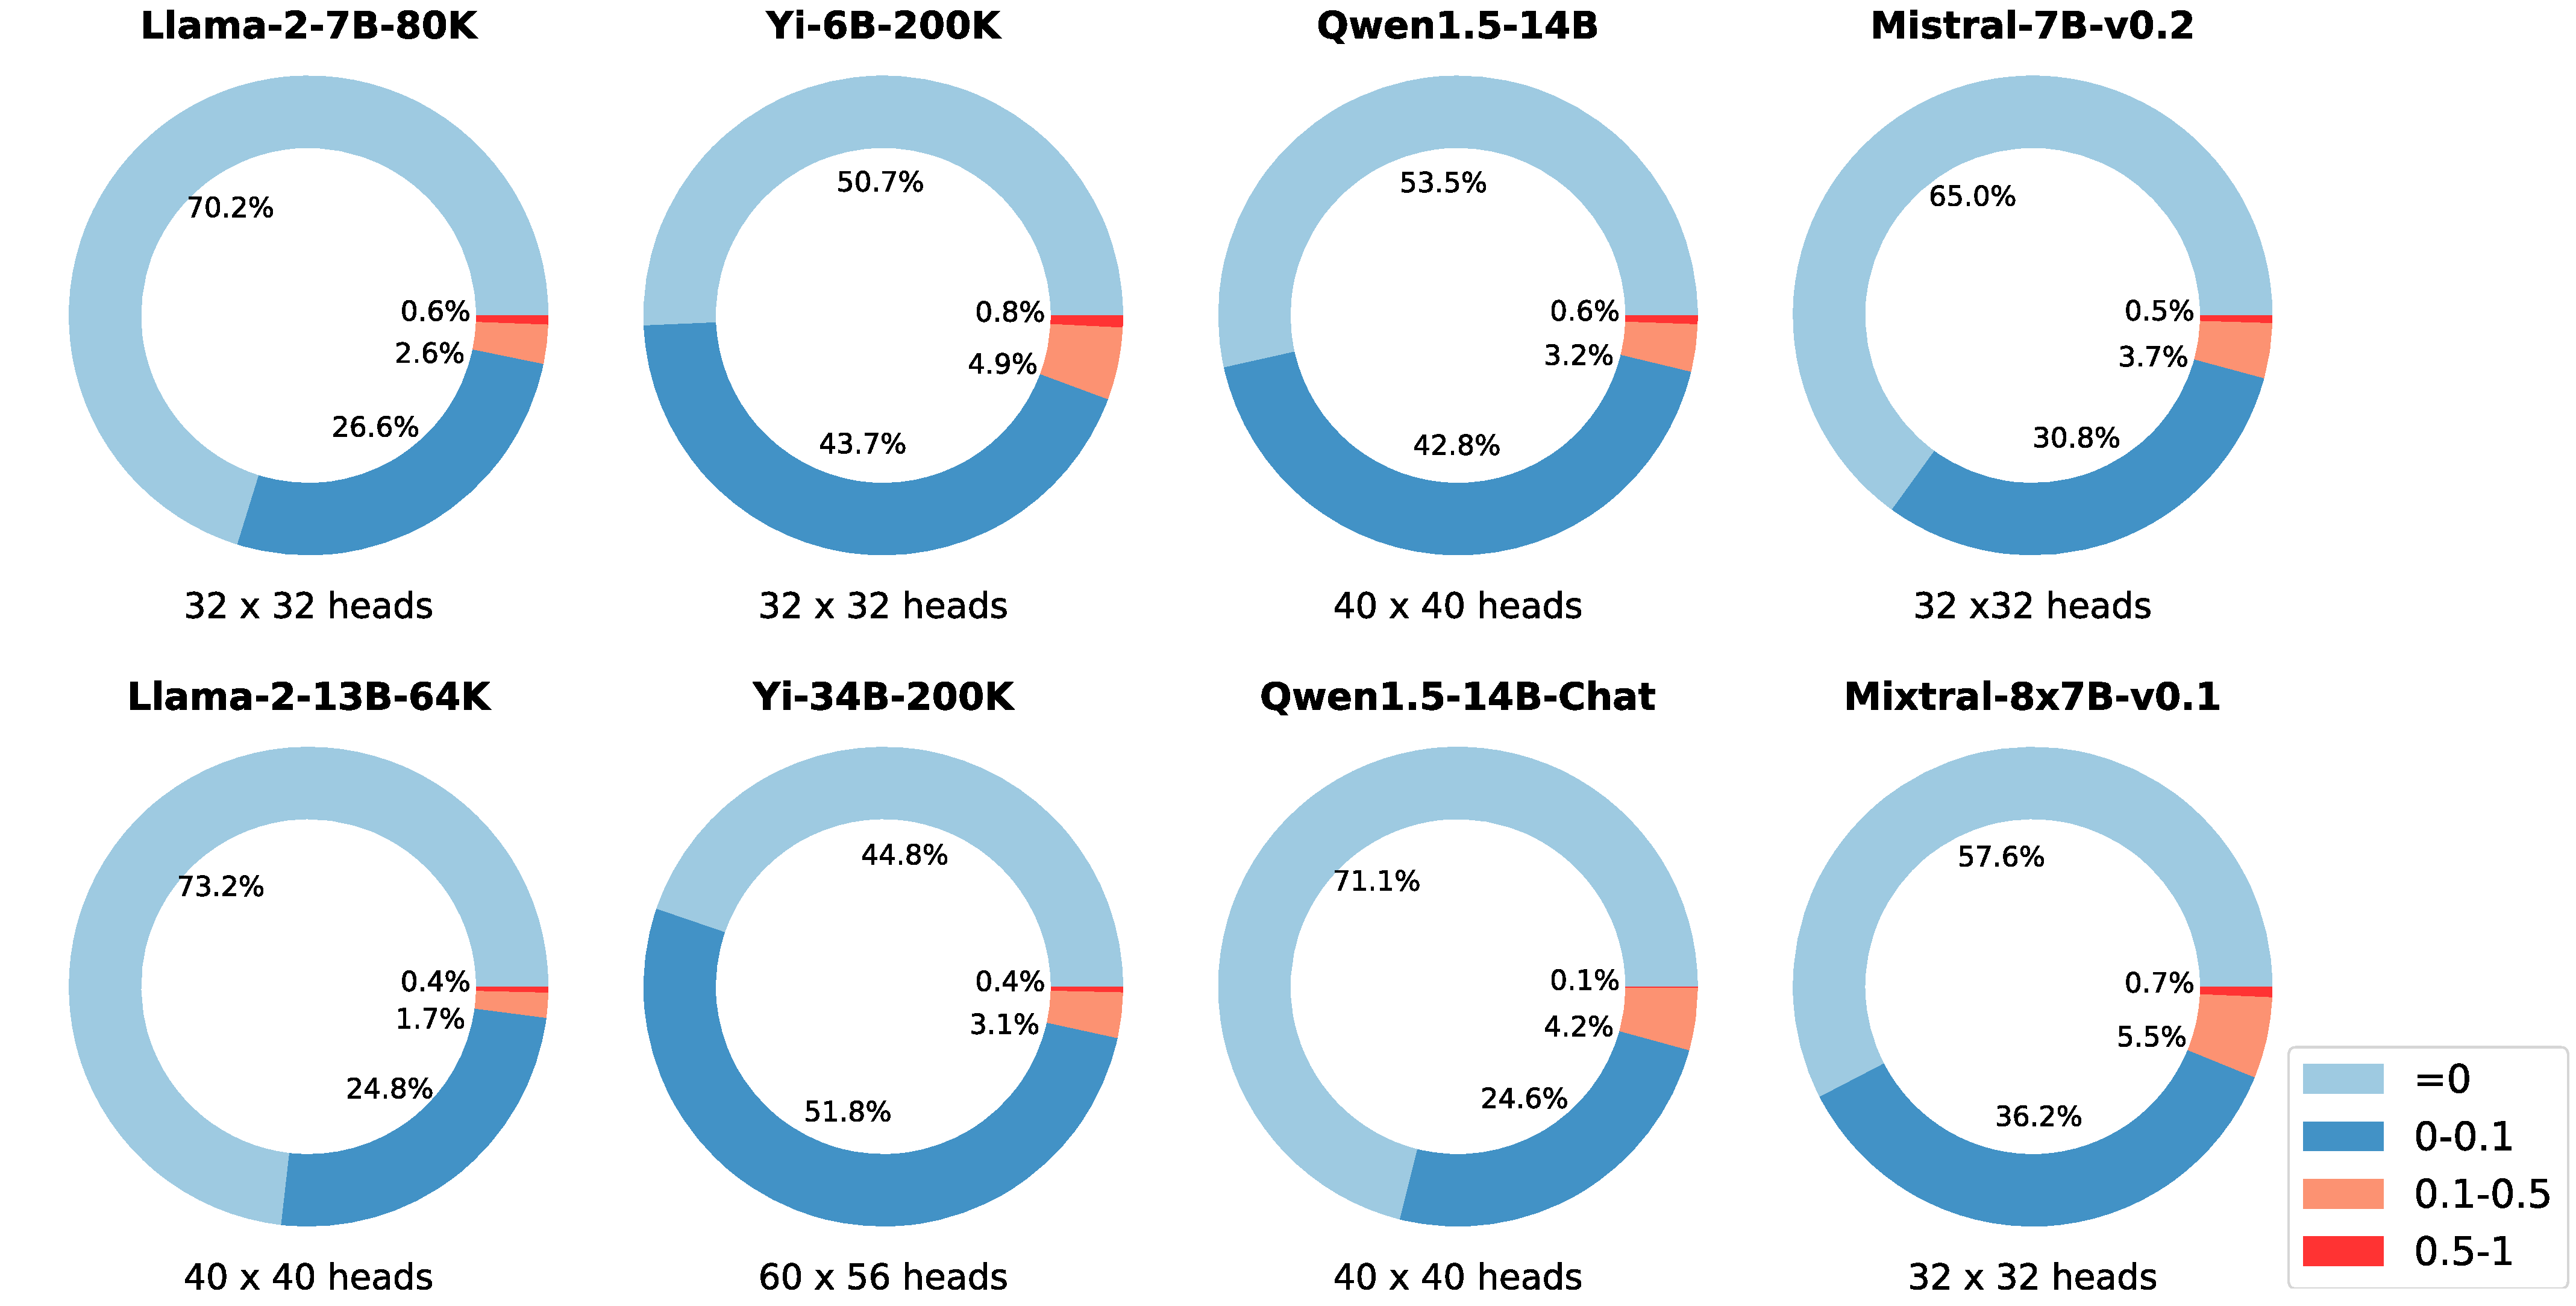
\includegraphics[width=\linewidth]{figures/ring_graph.pdf}
  \caption{Retrieval heads are universal and sparse across model family and scale. 
  For all models we consider, less than 5\% of the attention heads are activated more than 50\% of the time (with a retrieval score higher than 0.5) when retrieval is required.
  }
  \label{fig:score_range}
\end{figure*}


This section discusses important properties of retrieval heads:
(1) universal and sparse: any model that exhibits long-context capability has a small set of retrieval heads;
(2) dynamic: most of retrieval heads are activated under different contexts;
(3) intrinsic: retrieval heads are already within the base model as a consequence of large-scale pretraining. Subsequent models reuse the same set of heads. 
Our results are supported by extensive experiments on a large spectrum of models (Table~\ref{tab:all_models}).
To investigate the influence of continued pretraining for context length extension, we compare Llama-2-7B 4K to Llama-2-7B-80K and Llama-2-13B-60K \citep{fu2024data}. 
To examine the effect of alignment, we have study Mistral-7B-Instruct-v0.2 and Qwen-1.5-14B-Chat \citep{bai2023qwen} and compare them to their base versions.
We further choose Mixtral-8x7B-v0.1 \citep{jiang2024mixtral}, a mixture of expert versions derived from Mistral-7B-v0.2, presumably via sparse upcycling~\citep{komatsuzaki2022sparse}, to study retrieval heads in different architectures. 


\subsection{Universal and Sparse}
Figure~\ref{fig:score_range} demonstrate that a sparse set of retrieval heads exist in all models we consider, regardless of the various pertraining, fine-tuning recipes and the underlying architecture.
Between 25\% and 52\% of the heads exhibit copy-paste behaviors at a very low frequency, with a score of between 0 and 0.1. 
Approximately 45\% to 73\% of attention heads have 0 retrieval score, meaning that they have other functionality than retrieval.
Only about 3\% to 6\% of the attention heads have a retrieval score larger than 0.1 (recall that a retrieval score 0.1 means a head retrieves at least 10\% of the tokens being asked).
It is also intriguing that although all model parameters, particularly the total number to attention heads, are largely different from each other, their ratio of retrieval heads lays in the same interval (about 5\%). 

\begin{figure*}[!t]
\small
  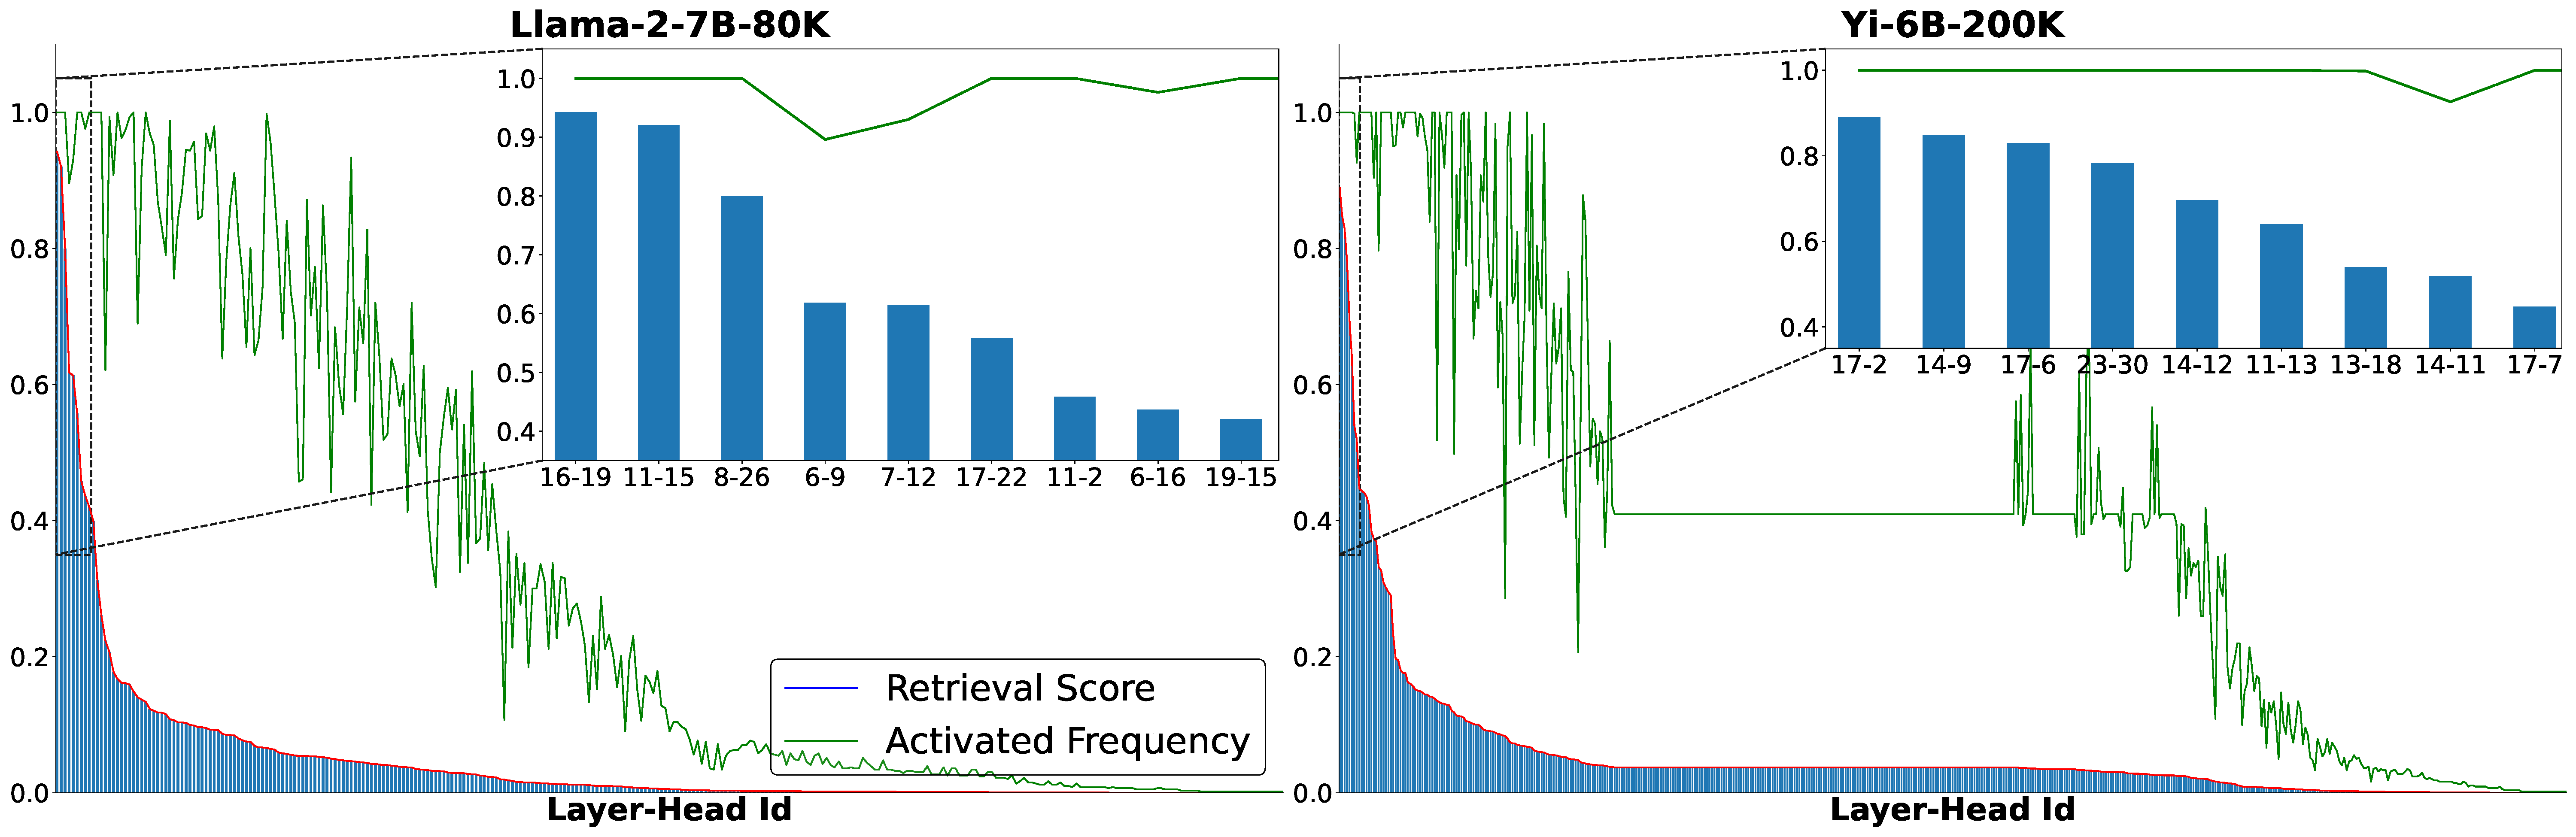
\includegraphics[width=\linewidth]{figures/score_distribution.pdf}
  \caption{Retrieval score (blue): average number of activated tokens; 
  Activation Frequency (green): frequency of at least activated on one token. 
  The \textit{gap} between the two curves shows \textit{context-sensitivity}: a head of high activation frequency but low retrieval score means it is only activated on certain tokens and contexts; a head of high retrieval score means it is activated on almost any context. 
  For both LLaMA and Yi, there exist strong heads that are not sensitive to context and always activated.
  }
  \label{fig:score_dist}
\end{figure*}


\subsection{Dynamically Activated Based on Tokens and Contexts}
Now we study how sensitive a retrieval head is to its input context, i.e.,
whether a head is consistently activated no matter what the context is, or if a head is activated only on specific contexts.
For the needle sentences "the best thing to do in San Francisco is eating a sandwich in Dolores park in a sunny day", some heads are activated on the full sentence, whereas other heads  only activated on certain tokens like ``eating a sandwich'' or ``in Dolores park'. 
We define \textit{activation frequency}, the frequency of a head being activated on \textit{at least one token} (v.s., the retrieval score measures the \textit{average} number of activated tokens). 
A head of high activation frequency but low retrieval score means it is only activated on certain tokens and contexts.
As is shown in Fig.~\ref{fig:score_dist}, 
Llama-2-7B-80K and Yi-6B-200K have 12 and 36 strongest retrieval heads, respectively, that are always activated (activation frequency equal to 1) under all the contexts we consider. 
Weaker heads only activate on certain tokens and contexts. 


\subsection{Intrinsic}
\begin{figure*}[t!]
\small
  \centering
  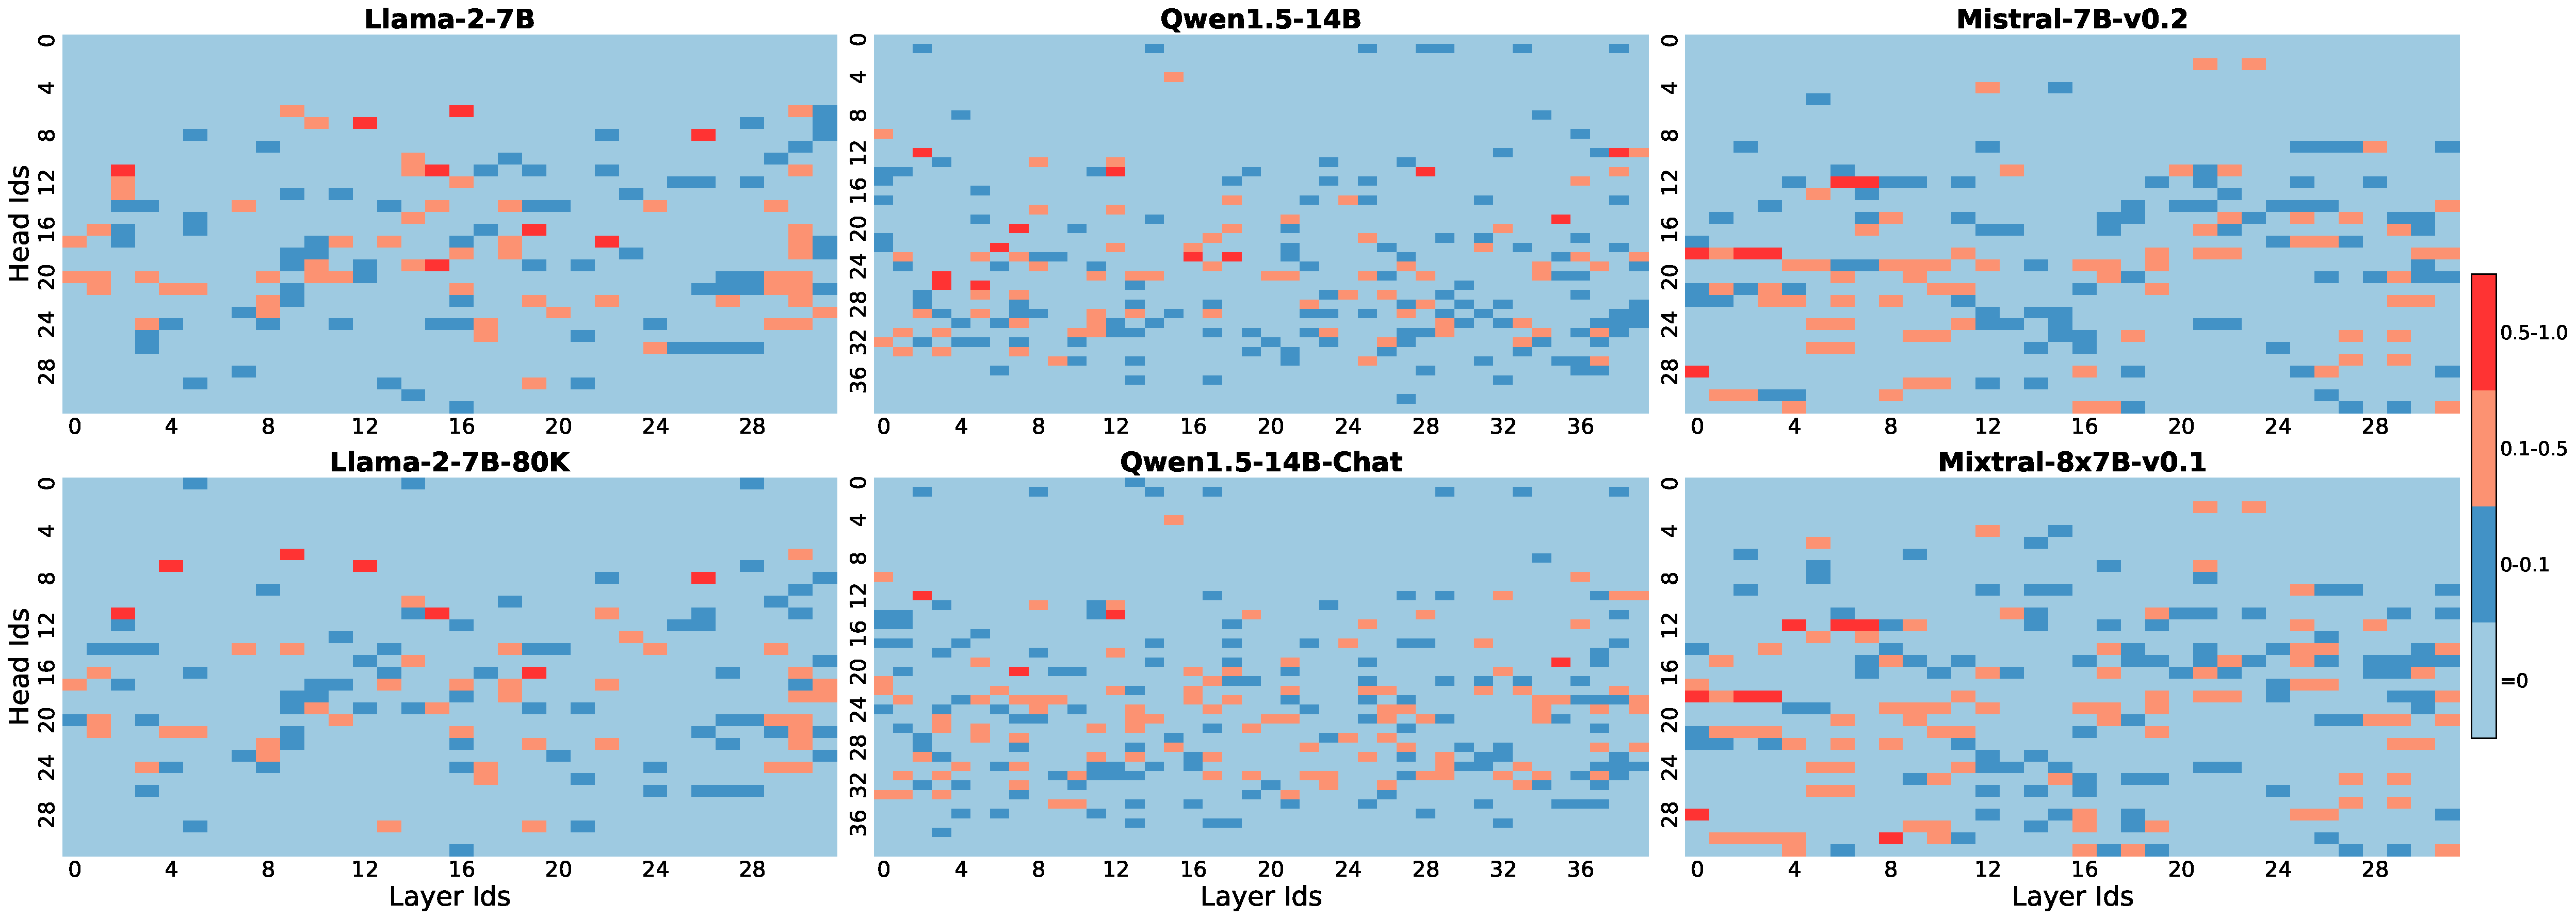
\includegraphics[width=\linewidth]{figures/heat_map.pdf}
\caption{Retrieval head is intrinsic and already within the base model. The subsequent model derivations, either by continue pretraining (LLaMA 2 7B 80K) or chat finetuning (Qwen 1.5 14B Chat) or sparse upcycling (Mixtral 8$\times$7B), use the same set of retrieval head as the base model, as demonstrated by a high level of similarity between the heatmap patterns. 
}
  \label{fig:heat_map}
\end{figure*}

We show that the retrieval heads, thus the ability of utilizing information at arbitrary location of the input, is an intrinsic property~\citep{fu2024data} of the base model as a consequence of large-scale pretraining, with subsequent small-scale training exerting only minor alterations to these head activation patterns.
In Figure~\ref{fig:heat_map}, we present the retrieval score distributions for a range of base models in the initial row, followed by their corresponding variants in the subsequent row. We see that regardless of the models being continuously pre-trained, chat fine-tuned, or sparsely upcycled, there is a notable consistency in their retrieval scores heatmaps. 
Figure~\ref{fig:corr_map} offers a more direct and strict examination, where we compute the statistical correlations between different models. 
The data reveal a high degree of correlation in the retrieval score distributions between base models and their respective variants, with a Pearson correlation coefficient exceeding 0.8. 
Models from different families exhibit a correlation coefficient of less than 0.1, indicative of their distinct pretraining recipes.

\begin{figure}[!t]
    \begin{minipage}[!t]{0.48\textwidth}
        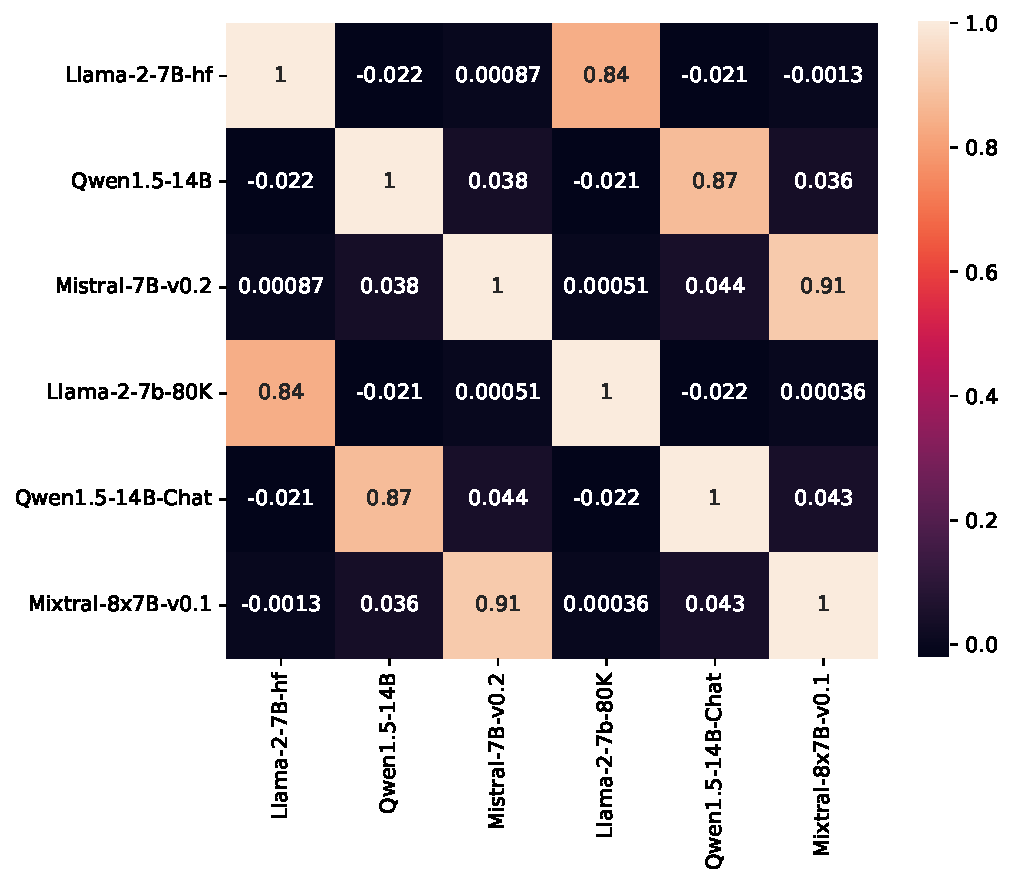
\includegraphics[width=\textwidth]{figures/corr_map.pdf}
        \caption{The retrieval heads of models of the same family are strongly correlated, i.e., the chat model and base model typically uses the same set of retrieval heads.
        The retrieval heads of models of different families are clearly different. 
        % For models of different families, their retrieval heads are clearly different. 
        }
        \label{fig:corr_map}
    \end{minipage}
    \hfill
    \begin{minipage}[t!]{0.48\textwidth}
        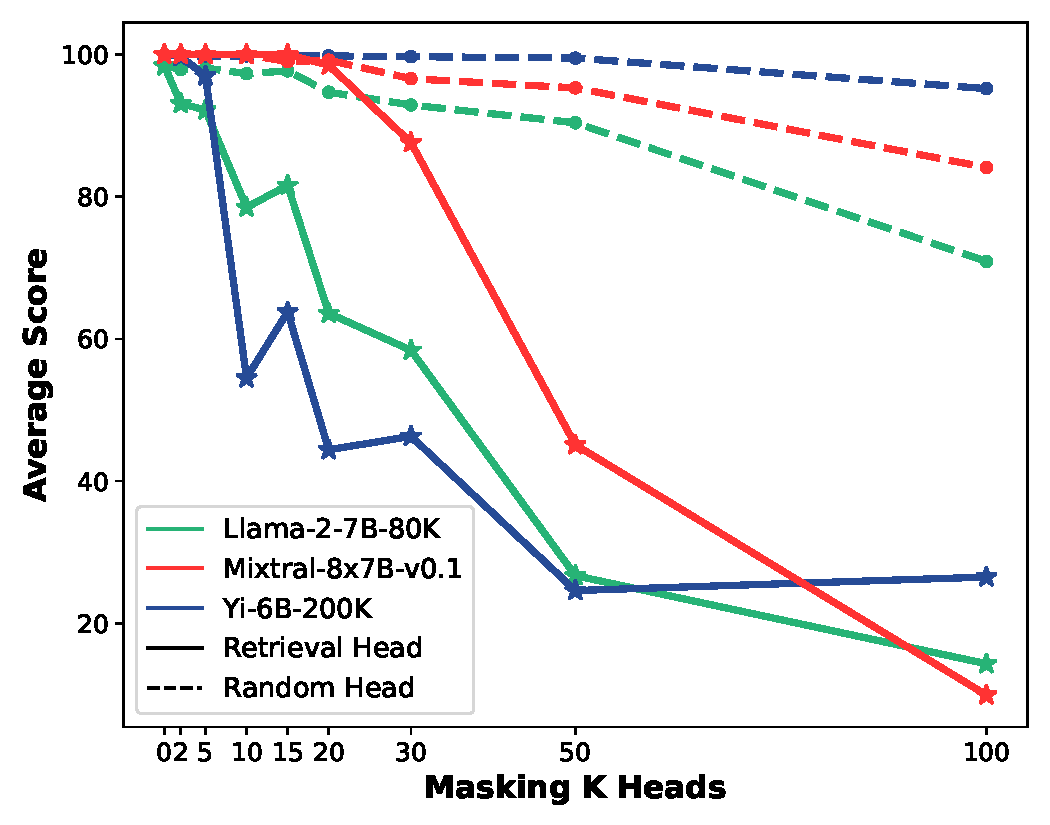
\includegraphics[width=\textwidth]{figures/masking_heads.pdf}
        \caption{Masking out top K retrieval heads vs K random heads. For all models are consider, the removal of retrieval heads clearly reduces the Needle-in-a-Haystack performance, versus the removal of non-retrieval heads have much weaker influence. 
        }
        \label{fig:needle_mask}
    \end{minipage}
\end{figure}




